% arara: pdflatex
% arara: pdflatex
% arara: pdflatex
% ----------------------------------------------------------------------------
% the XSIM package
% 
%   eXercise Sheets IMproved
% 
% ----------------------------------------------------------------------------
% Clemens Niederberger
% Web:    https://github.com/cgnieder/xsim
% E-Mail: contact@mychemistry.eu
% ----------------------------------------------------------------------------
% Copyright 2017 Clemens Niederberger
% 
% This work may be distributed and/or modified under the
% conditions of the LaTeX Project Public License, either version 1.3
% of this license or (at your option) any later version.
% The latest version of this license is in
%   http://www.latex-project.org/lppl.txt
% and version 1.3 or later is part of all distributions of LaTeX
% version 2005/12/01 or later.
% 
% This work has the LPPL maintenance status `maintained'.
% 
% The Current Maintainer of this work is Clemens Niederberger.
% ----------------------------------------------------------------------------
% If you have any ideas, questions, suggestions or bugs to report, please
% feel free to contact me.
% ----------------------------------------------------------------------------
\documentclass[load-preamble+]{cnltx-doc}
\usepackage[utf8]{inputenc}
\usepackage{xsim}

\xsimsetup{
  path = exercises
}

\setcnltx{
  package  = {xsim},
%  info     = {comprehensive support for typesetting chemistry documents},
  url      = https://github.com/cgnieder/xsim ,
  authors  = Clemens Niederberger ,
  email    = contact@mychemistry.eu ,
  abstract = {%
    \centering
    \par
  } ,
  quote-format = \small\biolinumLF ,
  add-silent-cmds = {lipsum} ,
  add-cmds = {
    blank ,
    collectexercises ,
    collectexercisestype ,
    collectexercisesstop ,
    DeclareExerciseCollection ,
    DeclareExerciseEnvironmentTemplate ,
    DeclareExerciseGoal ,
    DeclareExerciseHeadingTemplate ,
    DeclareExerciseProperty ,
    DeclareExercisePropertyAlias ,
    DeclareExerciseTableTemplate ,
    DeclareExerciseTagging ,
    DeclareExerciseTranslation ,
    DeclareExerciseTranslations ,
    DeclareExerciseType ,
    ExerciseID ,
    ExerciseGoalName ,
    ExerciseParameterGet ,
    ExercisePropertyGet ,
    ExercisePropertyGetAlias ,
    ExercisePropertyGlobalSave ,
    ExercisePropertyIfSetF ,
    ExercisePropertyIfSetT ,
    ExercisePropertyIfSetTF ,
    ExercisePropertySave ,
    ExercisyType ,
    ForeachExerciseTag ,
    ForEachExerciseTranslation ,
    ForEachPrintedExerciseByType ,
    ForEachPrintedExerciseByID ,
    ForEachUsedExerciseByType ,
    ForEachUsedExerciseByID ,
    GetExerciseAliasProperty ,
    GetExerciseName ,
    GetExerciseParameter ,
    GetExerciseProperty ,
    GlobalSaveExerciseProperty ,
    gradingtable ,
    IfExerciseGoalF ,
    IfExerciseGoalF ,
    IfExerciseGoalTF ,
    IfExercisePropertyExistF ,
    IfExercisePropertyExistT ,
    IfExercisePropertyExistTF ,
    IfExercisePropertySetF ,
    IfExercisePropertySetT ,
    IfExercisePropertySetTF ,
    IfInsideSolutionF ,
    IfInsideSolutionT ,
    IfInsideSolutionTF ,
    printcollection ,
    printsolutions ,
    printsolutionstype ,
    SaveExerciseProperty ,
    SetExerciseParameter ,
    SetExerciseParameters ,
    TotalExerciseGoal ,
    TotalExerciseTypeGoal ,
    UseExerciseTags ,
    UseExerciseTagsX ,
    XSIMexpandcode ,
    XSIMifblankT ,
    XSIMifblankF ,
    XSIMifblankTF ,
    XSIMifeqF ,
    XSIMifeqT ,
    XSIMifeqTF ,
    XSIMmixedcase ,
    XSIMputright ,
    xsimsetup ,
    XSIMtranslate
  } ,
  add-envs = { exercise , solution } ,
  add-silent-cmds = {
  } ,
  index-setup = { othercode = \footnotesize , level = \section } ,
  makeindex-setup = { columns = 2 , columnsep = 1em } ,
  add-frame-options = { skipabove = 0pt , skipbelow = 0pt }
}

\expandafter\def\csname libertine@figurestyle\endcsname{LF}
\usepackage[libertine]{newtxmath}
\expandafter\def\csname libertine@figurestyle\endcsname{OsF}

\newcommand*\eTeX{%
  \texorpdfstring
    {\mbox{$\epsilon$-\TeX}}
    {e-TeX}%
}

\usepackage[biblatex]{embrac}
\ChangeEmph{[}[,.02em]{]}[.055em,-.08em]
\ChangeEmph{(}[-.01em,.04em]{)}[.04em,-.05em]

\makeatletter
\colorlet{property}{orange}
\newidxcmd\property{\code{\textcolor{property}{#1}}}[ (property)]
\newrobustcmd*\prop{\@ifstar{\cnltx@prop@star}{\cnltx@prop@nostar}}

\newrobustcmd*\cnltx@prop@star{%
  \cnltx@ifdash
    {\cnltx@prop@aux*\meta}
    {\cnltx@prop@aux*\marg}%
}
\newrobustcmd*\cnltx@prop@nostar{%
  \cnltx@ifdash
    {\cnltx@prop@aux{}\meta}
    {\cnltx@prop@aux{}\marg}%
}
\newcommand*\cnltx@prop@aux[4]{%
  \code{\property#1{#3}\cnltx@isvalue#2{#4}}%
}

\newrobustcmd*\propis{%
  \@ifstar
    {\cnltx@propis*}
    {\cnltx@propis{}}%
}
\newrobustcmd*\cnltx@propis[1]{%
  \cnltx@ifdash
    {\cnltx@prop@aux{#1}\@firstofone}
    {\cnltx@prop@aux{#1}\Marg}%
}
\newrobustcmd*\choiceprop{%
  \@ifstar
    {\cnltx@choiceprop@star}
    {\cnltx@choiceprop@nostar}%
}
\def\cnltx@choiceprop@star#1#2{%
  \code{\property*{#1}\cnltx@isvalue\choices{#2}}}
\def\cnltx@choiceprop@nostar#1#2{%
  \code{\property{#1}\cnltx@isvalue\choices{#2}}}
\newcommand*\boolprop{%
  \@ifstar
    {\cnltx@boolprop@star}
    {\cnltx@boolprop@nostar}%
}
\def\cnltx@boolprop@star#1{\choiceprop*{#1}{\default{true},false}}
\def\cnltx@boolprop@nostar#1{\choiceprop{#1}{\default{true},false}}

\newenvironment{properties}
  {%
    \def\propert{\@cnltx@option@item\property}%
    \def\propval{\@cnltx@option@item\prop}%
    \def\proplit{\@cnltx@option@item\propis}%
    \def\propchoice{\@cnltx@option@item\choiceprop}%
    \def\propbool{\@cnltx@option@item\boolprop}%
    \cnltxlist
  }
  {\endcnltxlist}

\colorlet{parameter}{blue}
\newidxcmd\parameter{\code{\textcolor{parameter}{#1}}}[ (parameter)]
\newrobustcmd*\para{\@ifstar{\cnltx@para@star}{\cnltx@para@nostar}}

\newrobustcmd*\cnltx@para@star{%
  \cnltx@ifdash
    {\cnltx@para@aux*\meta}
    {\cnltx@para@aux*\marg}%
}
\newrobustcmd*\cnltx@para@nostar{%
  \cnltx@ifdash
    {\cnltx@para@aux{}\meta}
    {\cnltx@para@aux{}\marg}%
}
\newcommand*\cnltx@para@aux[4]{%
  \code{\parameter#1{#3}\cnltx@isvalue#2{#4}}%
}

\newrobustcmd*\parais{%
  \@ifstar
    {\cnltx@parais*}
    {\cnltx@parais{}}%
}
\newrobustcmd*\cnltx@parais[1]{%
  \cnltx@ifdash
    {\cnltx@para@aux{#1}\@firstofone}
    {\cnltx@para@aux{#1}\Marg}%
}
\newrobustcmd*\choicepara{%
  \@ifstar
    {\cnltx@choicepara@star}
    {\cnltx@choicepara@nostar}%
}
\def\cnltx@choicepara@star#1#2{%
  \code{\parameter*{#1}\cnltx@isvalue\choices{#2}}}
\def\cnltx@choicepara@nostar#1#2{%
  \code{\parameter{#1}\cnltx@isvalue\choices{#2}}}
\newcommand*\boolpara{%
  \@ifstar
    {\cnltx@boolpara@star}
    {\cnltx@boolpara@nostar}%
}
\def\cnltx@boolpara@star#1{\choicepara*{#1}{\default{true},false}}
\def\cnltx@boolpara@nostar#1{\choicepara{#1}{\default{true},false}}

\newenvironment{parameters}
  {%
    \def\param{\@cnltx@option@item\parameter}%
    \def\paraval{\@cnltx@option@item\para}%
    \def\paralit{\@cnltx@option@item\parais}%
    \def\parachoice{\@cnltx@option@item\choicepara}%
    \def\parabool{\@cnltx@option@item\boolpara}%
    \cnltxlist
  }
  {\endcnltxlist}

\makeatother

\usepackage{acro}

\DeclareAcronym{prop}{
  short = property ,
  long  = \emph{Properties} are options of exercises which are individual for
    each exercise and can be retrieved and used in exercise templates. ,
  short-plural-form = properties
}

\DeclareAcronym{para}{
  short = parameter ,
  long  = \emph{Parameters} are options of exercise types which are the same
    for each exercise of a type and can be retrieved and used in exercise
    templates.
}

\DeclareAcronym{goal}{
  short = goal ,
  long  = \emph{Goals} are a certain type of \acsp*{prop} with a numerical
    value the sum of which is available throughout the document.
}

\DeclareAcronym{tag}{
  short = tag ,
  long  = \emph{Tags} are a certain type of \acsp*{prop} with a csv list as
    value which can be used for selective usage of exercises.
}

\DeclareAcronym{coll}{
  short = collection ,
  long  = A \emph{collection} bundles a number of exercises of one type or all
    types of exercises within certain barriers in the document.  Those
    exercise collections can be printed at any place in the document
    \emph{after} the collection is complete.
}

\DeclareAcronym{tmpl}{
  short = template ,
  long  = {\emph{Templates} are generic code frameworks which are used for
    typesetting \xsim's objects such as exercises, solutions, or grading
    tables.}
}

\ExplSyntaxOn
\NewAcroCommand \Acs
  {
    \acro_first_upper:
    \acro_short:n {#1}
  }
\NewAcroCommand \Acsp
  {
    \acro_first_upper:
    \acro_plural:
    \acro_short:n {#1}
  }
\ExplSyntaxOff

\newcommand\environ[1]{\beginenv*\Marg{\env{exercise}}}

\DeclareExerciseCollection{foo}

\usepackage{lipsum}
\usepackage{varioref}

\begin{document}

\section{Licence, Requirements and \textsc{README}}
\license

\xsim\ loads the packages \pkg{expl3}~\cite{bnd:l3kernel},
\pkg{xparse}~\cite{bnd:l3packages}, \pkg{etoolbox}~\cite{pkg:etoolbox},
\pkg{booktabs}~\cite{pkg:booktabs} and
\pkg{translations}~\cite{pkg:translations}.  All of these packages are present
on a modern and up to date \TeX\ distribution such as \TeX~Live or MiK\TeX\ so
no further action should be needed.

\section{Motivation and Background}

It has been quite a while since I first published
\pkg{exsheets}~\cite{pkg:exsheets} in Juni 2012.  Since then it has gained a
user base and a little bit of popularity as the number of questions on tex.sx
shows (98~at the time of writing).  User questions, bug reports and feature
requests improved it over the time.  It still has a version number starting
with a zero, though, which in my versioning system means I still consider it
experimental.

This is due to several facts.  It lacks a few features which I consider
essential for a full version~1.  For one thing it is not possible to have
several kinds of exercises numbered independently.  Using verbatim material
such as listings inside exercises and solutions is not possible and the
current workaround isn't that ideal either.  One request which dates back
quite a while now was to have different types of points to exercises\ldots

All of those aren't easy to add due to the way \pkg{exsheets} is implemented
right now. As a consequence I wanted to re-implement \pkg{exsheets} for a long
time.  This is what lead to \xsim.  Internally the package works completely
different. It will be the official successor of \pkg{exsheets} which is now
considered obsolete and will only receive bugfix releases any more.

\section{Package Options}\label{sec:package-options}
\xsim\ has two package options:
\begin{options}
  \opt{verbose}
    Writes extensive information about what \xsim\ is doing into the log
    file.
  \opt{final}
    If used the exercise and solution environments will not rewrite the
    environment body files.
\end{options}

Those options are used the usual way as package option
\begin{sourcecode}
  \usepackage[verbose]{xsim}
\end{sourcecode}
or as global option
\begin{sourcecode}
  \documentclass[verbose]{article}
\end{sourcecode}
or via the setup command:
\begin{commands}
  \command{xsimsetup}[\marg{options}]
    Set up \xsim's two package options and all other options described at
    other places in the manual.
\end{commands}

\section{How to Read the Manual}\label{sec:how-read-manual}

\subsection{Nomenclature}

Throughout this manual certain terms are used.  This section explains their
meaning in this manual.

\acuseall
\printacronyms[heading=none]

\subsection{Setting Options}
Apart from the package options already described in
section~\vref{sec:package-options} \xsim\ has further options. Those can be
\enquote{toplevel} options or options belonging to a module.
\begin{options}
  \keyval*{toplevel}{value}
    A toplevel option.
  \keyval*{sublebel}{value}\Module*{module}
    A sublevel option belonging to the module \module*{module}
\end{options}
Both kinds of options are set with \cs{xsimsetup}:
\begin{sourcecode}
  \xsimsetup{
    toplevel = {value} ,
    module/sublevel = {value}
  }
\end{sourcecode}

\subsection{Command descriptions}

Some commands do have a \expandablesymbol\ symbol printed next to their
names.  This indicates that the command is expandable, \ie, it is usable in an
\cs*{edef} or \cs*{write} context and will expand according to its
description.  All other commands are engine protected, \ie, in the sense of
\eTeX's \cs*{protected}.

\section{Exercises and Solutions}

\subsection{The Environments}

\begin{environments}
  \environment{exercise}[\oarg{\acsp*{prop}}]
    Input and typeset an exercise.  See section~\vref{sec:exercise-properties}
    for details on exercise \acsp*{prop}.
  \environment{solution}[\oarg{options}]
    Input and typeset the solution to the exercise of the previous
    \env{exercise} environment.  See section~\vref{sec:printing-solutions} for
    details on options of solutions.
\end{environments}

\begin{example}
  \begin{exercise}
    A first example for an exercise.
  \end{exercise}
  \begin{solution}
    A first example for a solution.
  \end{solution}
\end{example}

As can be seen in the example a solution is not printed with the default
setup.  This can be changed using the following option.
\begin{options}
  \keybool{print}\Module{solution}\Default{false}
    Set if solutions are printed or or not.
\end{options}

The option (belonging to the module \module*{solution}) can either be set
locally as option to the \env{solution} environment
\begin{sourcecode}
  \begin{solution}[print=true]
    A first example for a solution.
  \end{solution}
\end{sourcecode}
or with the setup command for all following solutions:
\begin{sourcecode}
  \xsimsetup{
    solution/print = true
  }
\end{sourcecode}

There is an completely analoguous option for the \env{exercise} environment:
\begin{options}
  \keybool{print}\Module{exercise}\Default{true}
    Set if exercises are printed or or not.
\end{options}
See also section~\vref{sec:using-printing}.

\section{How the Exercise Environments Work}
Both enviroments write the contents of their bodies verbatim to external files
following a certain naming structure:
\begin{itemize}
  \item
  \code{\meta{jobname}-\meta{type}-\meta{id}-exercise|solution-body.tex} 
\end{itemize}
The name starts with the name of the job (which is the name of the document
itself) followed by type and id of the corresponding exercise and then
followed by the environment type.  For example both enviroments from the first
example have been written to files named
\begin{itemize}
  \item \verbcode+xsim_manual-exercise-1-exercise-body.tex+ and
  \item \verbcode+xsim_manual-exercise-1-solution-body.tex+, respectively.
\end{itemize}
Details on the \meta{type} of an exercise will be given in
section~\vref{sec:new-exercise-types}.  \emph{The \meta{id} of an exercise is
  a positive integer unique to each exercise environment regardless if the
  exercise is being printed or used at all.}

These external files are input when the respective exercise or solution is
printed.  An advantage of using external files is that \emph{verbatim material
  is allowed} inside the environments.  Each of those files contains some
information about itself and where and why it was generated\footnote{In this
  example the sourcecode line number is misleading as the example where the
  file was generated itself was an external file where the \env{exercise}
  environment indeed \emph{was} on line~1.}:

\inputsourcecode{exercises/xsim_manual-exercise-1-exercise-body.tex}

Arguably one downside of the approach using external files for each exercise
and its solution is that your project folder will be cluttered with files.  In
order to deal with this somehow \xsim\ offers the following option:
\begin{options}
  \keyval{path}{path name}\Default
    With this option a subfolder or path within the main project folder can be
    given.  Exercises will be written to and included from this path.
    \emph{The path must exist on your system before you can use it!} This
    document uses \keyis{path}{exercises}.
\end{options}

\section{New Exercise Types}\label{sec:new-exercise-types}

It is easy to define new exercise environments together with a corresponding
solution environment using the following command:
\begin{commands}
  \command{DeclareExerciseType}[\marg{type}\marg{parameters}]
    Declare a new exercise type analoguous to the \env{exercise} and
    \env{solution} environments.
\end{commands}

The existing environment pair has been defined as follows:
\begin{sourcecode}
  \DeclareExerciseType{exercise}{
    exercise-env      = exercise ,
    solution-env      = solution ,
    exercise-name     = \XSIMtranslate{exercise} ,
    solution-name     = \XSIMtranslate{solution} ,
    exercise-template = subsection* ,
    solution-template = subsection*
  }
\end{sourcecode}

The above already is an example for almost all parameters that can (and often
must) be set.  Here is the complete list:
\begin{parameters}
  \paraval{exercise-env}{exercise environment name}
    The name for the environment used for the exercises of type \meta{type}.
    \emph{This parameter must be set.}
  \paraval{solution-env}{solution environment name}
    The name for the environment used for the solutions of type \meta{type}.
    \emph{This parameter must be set.}
  \paraval{exercise-name}{exercise name}
    The name of the exercises of type \meta{type} -- used for typesetting.
    \emph{This parameter must be set.}
  \paraval{solution-name}{solution name}
    The name of the solutions of type \meta{type} -- used for typesetting.
    \emph{This parameter must be set.}
  \paraval{exercise-template}{exercise template}
    The template used for typesetting the exercises of type \meta{type}.
    \emph{This parameter must be set.} See section~\vref{sec:styl-exerc-templ}
    for details on templates.
  \paraval{solution-template}{solution template}
    The template used for typesetting the exercises of type \meta{type}.
    \emph{This parameter must be set.} See section~\vref{sec:styl-exerc-templ}
    for details on templates.
  \paraval{counter}{counter name}
    The counter used for the exercises of type \meta{type}.  If not explicitly
    set the counter with the same name as \parameter{exercise-env} is used.
    Otherwise the specified counter is used.  This enables to have different
    types of exercises sharing a common counter.
\end{parameters}

It is possible to change some parameters after an exercise type has been
defined.  Those include \parameter{exercise-name}, \parameter{solution-name},
\parameter{exercise-template}, \parameter{solution-template}, and
\parameter{counter}:
\begin{commands}
  \command{SetExerciseParameter}[\marg{type}\marg{parameter}\marg{value}]
    Usable to set a single parameter to a new value.
  \command{SetExerciseParameters}[\marg{type}\marg{parameters}]
    Set several parameters at once. \meta{parameters} is a csv list of
    key/value pairs.
\end{commands}
If you try to set and already set but fixed parameter like
\parameter{exercise-env} a warning will be written to the log file.  If you
set \parameter{counter} to another value you must make sure that the new value
is a valid and defined counter.

\section{Exercise Properties}\label{sec:exercise-properties}

\subsection{Predefined Properties}

Exercise like the \env{exercise} environment and possibly others defined with
\cs{DeclareExerciseType} have a number of predefined \acsp*{prop}:
\begin{properties}
  \propval{id}{integer}
    Holds the internal id of an exercise.  \emph{Cannot be set by the user}.
  \propval{ID}{text}
    Holds the user id of an exercise if defined.  Otherwise it is equal to
    \property{id}.
  \propval{counter}{integer}
    Holds the counter value of an exercise.  \emph{Cannot be set by the
      user}.
  \propval{subtitle}{text}
    Holds the subtitle of an exercise.
  \propval{points}{number}
    Holds the reachable points of an exercise.
  \propval{bonus-points}{number}
    Holds the reachable bonus-points of an exercise.
  \propbool{print}
    Holds the print boolean of an exercise.
  \propbool{use}
    Holds the usage boolean of an exercise.
  \propval{tags}{csv list of tags}
    Holds the list of tags the exercise should be associated with.
  \propval{topics}{csv list of topics}
    Holds the list of topics the exercise should be associated with.
\end{properties}

Some of these \acsp*{prop} are fixed and cannot be set by the user.  Those
include \property{id} and \property{counter}.  The others can be set using the
optional argument of the exercise environment.

\begin{example}
  \begin{exercise}[subtitle={This is a subtitle}]
    An exercise where some properties have been set.
  \end{exercise}
\end{example}

\subsection{Declaring Own Properties}

\xsim\ offers the possibility to declare additional exercise properties:
\begin{commands}
  \command{DeclareExerciseProperty}[\sarg\marg{property}]
    Declares the property \meta{property}.  If used with the optional star a
    unique property is defined which means that each exercise must have a
    property value distinct from all other exercises.
  \command{DeclareExercisePropertyAlias}[\marg{property 1}\marg{property 2}]
    Declares \meta{property 1} to be an alias of \meta{property 2}.  This
    means that each time \meta{property 2} is set \meta{property 1} will be
    set to the same value \emph{unless} it has been set already.  As an
    example: property \property{ID} is an alias of property \property{id}.
\end{commands}

This is better demonstrated with an example:
\begin{example}
  \begin{exercise}
    \lipsum[4] % from package `lipsum'
    \verb+\GetExerciseProperty{id}+: \GetExerciseProperty{id} \par
    \verb+\GetExerciseAliasProperty{ID}+: \GetExerciseAliasProperty{ID} \par
    \verb+\GetExerciseProperty{ID}+: \GetExerciseProperty{ID}
  \end{exercise}
  \begin{exercise}[ID=foo-bar]
    \lipsum[4]
    \verb+\GetExerciseProperty{id}+: \GetExerciseProperty{id} \par
    \verb+\GetExerciseAliasProperty{ID}+: \GetExerciseAliasProperty{ID} \par
    \verb+\GetExerciseProperty{ID}+: \GetExerciseProperty{ID}
  \end{exercise}
\end{example}

The power of properties will get more clear when reading
section~\vref{sec:styl-exerc-templ} about templates.

\subsection{A Special Kind of Property: Exercise Goals}

Exercise goals are a generic concept in \xsim\ for exercise properties like
\property{points} or \property{bonus-points}.  Those are properties which can
(only) get a decimal number as value the sum of which is calculated and
available (after a compilation) throughout the document.
\begin{commands}
  \command{DeclareExerciseGoal}[\marg{goal}]
    Declare a new exercise goal named \meta{goal} and also a property called
    \meta{goal}.
  \command{TotalExerciseTypeGoal}[\marg{type}\marg{goal}\marg{singular}\marg{plural}]
    Get the sum of goal \meta{goal} for all exercises of type \meta{type}.
    \meta{singular} andf \meta{plural} are placed after the sum in the input
    stream depending on whether the sum equals~$1$ or not.
  \command{TotalExerciseGoal}[\marg{goal}\marg{singular}\marg{plural}]
    Get the sum of goal \meta{goal} for all exercises. \meta{singular} andf
    \meta{plural} are placed after the sum in the input stream depending on
    whether the sum equals~$1$ or not.
  \command{printpoints}[\marg{type}]
    Print the sum of points for all exercises of type \meta{type} followed by
    an appropriate translation of the words \enquote{point} or
    \enquote{points}, respectively\footnote{See section~\vref{sec:exerc-transl}
      for details on the definition and usage of language dependent words.}.
    Defined in terms of \cs{TotalExerciseTypeGoal}.
  \command{printtotalpoints}
    Print the sum of points for all exercises followed by an appropriate
    translation of the words \enquote{point} or \enquote{points},
    respectivaly.  Defined in terms of \cs{TotalExerciseGoal}.
  \command{printbonus}[\marg{type}]
    Print the sum of bonus points for all exercises of type \meta{type}
    followed by an appropriate translation of the words \enquote{point} or
    \enquote{points}, respectivaly.  Defined in terms of
    \cs{TotalExerciseTypeGoal}.
  \command{printtotalbonus}
    Print the sum of bonus points for all exercises followed by an appropriate
    translation of the words \enquote{point} or \enquote{points},
    respectivaly.  Defined in terms of \cs{TotalExerciseGoal}.
\end{commands}

The two existing goals are defined with
\begin{sourcecode}
  \DeclareExerciseGoal{points}
  \DeclareExerciseGoal{bonus-points}
\end{sourcecode}

\subsection{A Special Kind of Property: Exercise Tags}

Exercise tags are a generic concept in \xsim\ for exercise properties like
\property{tags} or \property{topics}.  Those are properties which can (only)
get a csv list of strings as value.  Those strings can be used to selectively
use exercises.  See section~\vref{sec:using-printing} for details on
\emph{usage} of exercises and the difference to \emph{printing} an exercise
and how to use exercise tags for selection.
\begin{commands}
  \command{DeclareExerciseTagging}{tag}
    This defines an exercise tagging group name \meta{tag}.  It also defines a
    property named \meta{tag}.  In addition to options are defines: and option
    named \code{\meta{tag}} which can be used for selection and an boolean
    option \code{\meta{tag}/ignore-untagged}.
\end{commands}
The two existing tagging groups have been defined and preset with the
following code:
\begin{sourcecode}
  \DeclareExerciseTagging{tags}
  \DeclareExerciseTagging{topics}
  \xsimsetup{tags/ingore-untagged=false}
\end{sourcecode}
this means that these options are available:
\begin{options}
  \keyval{tags}{csv list of tags}
    Choose the set of tags whose associated exercises should be printed.
  \keyval{topics}{csv list of topics}
    Choose the set of tags whose associated exercises should be printed.
  \keybool{ignore-tagging}\Module{tags}\Default{false}
    If set to true exercises with no tags will be printed even if tags have
    been chosen with the option \option{tags}.
  \keybool{ignore-tagging}\Module{topics}\Default{true}
    If set to true exercises with no topics will be printed even if tags have
    been chosen with the option \option{tags}.
\end{options}

\section{Using and Printing an Exercise}\label{sec:using-printing}

When an exercise is started with \environ{exercise} (or other environments
defined through \cs{DeclareExerciseType}) then different things happen
depending on different settings:
\begin{itemize}
  \item If the \emph{insert mode} is active nothing happens, see
    section~\vref{sec:collecting-exercises} for details on this.
  \item Else the id integer is incremented.
  \item If the exercise is \emph{used} the corresponding counter is stepped
    and the exercise is added to the \enquote{use list}.  The properties
    \property{counter} and \property{use} are updated accordingly.
  \item If an exercise is printed then it is also used. An exercise that isn't
    used cannot be printed.  Being printed means two things: being added to
    the \enquote{print list} and being typeset at the position where the
    exercise is placed in the source file.  If an exercise is \emph{not
      printed but used} it means that the counter will be stepped.  This can
    be useful for creating an exercise sheet only containing the solutions for
    some exercises.
  \item If an exercise is printed certain hooks and template code is inserted
    around the environment body.
\end{itemize}

\begin{example}[outside]
  \begin{exercise}[print=false]
    This exercise will not be printed but the exercise counter will be
    incremented nonetheless. Its solution will be printed in the list of
    solutions.
  \end{exercise}
  \begin{solution}
    The solution of the exercise that has not been printed.
  \end{solution}
\end{example}

The schematic structure of an exercise is shown in
figure~\vref{fig:schematic-structure}.

\begin{figure}
  \centering
  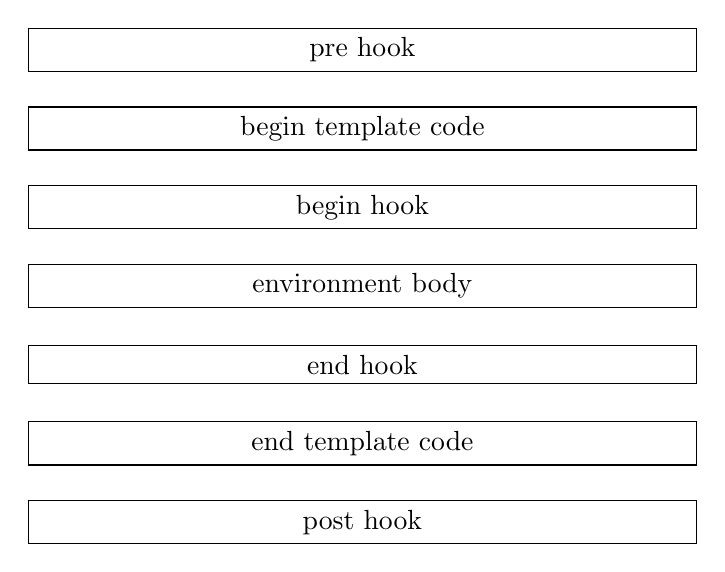
\begin{tikzpicture}
    \node[draw,minimum width=.7\linewidth] at (0,0)  {pre hook};
    \node[draw,minimum width=.7\linewidth] at (0,-1) {begin template code};
    \node[draw,minimum width=.7\linewidth] at (0,-2) {begin hook};
    \node[draw,minimum width=.7\linewidth] at (0,-3) {environment body};
    \node[draw,minimum width=.7\linewidth] at (0,-4) {end hook};
    \node[draw,minimum width=.7\linewidth] at (0,-5) {end template code};
    \node[draw,minimum width=.7\linewidth] at (0,-6) {post hook};
  \end{tikzpicture}
  \caption{Schematic structure of an exercise.}\label{fig:schematic-structure} 
\end{figure}

For each exercise type there are the following options (here using the
\module{exercise} type):
\begin{options}
  \keybool{print}\Module{exercise}\Default{true}
    Determines if exercises of type \module{exercise} are printed.
  \keybool{use}\Module{exercise}\Default{true}
    Determines if exercises of type \module{exercise} are used.
  \keyval{pre-hook}{code}\Module{exercise}\Default
    The code for the \emph{pre exercise hook} for exercises of the type
    \module{exercise}.
  \keyval{begin-hook}{code}\Module{exercise}\Default
    The code for the \emph{begin exercise hook} for exercises of the type
    \module{exercise}.
  \keyval{end-hook}{code}\Module{exercise}\Default
    The code for the \emph{end exercise hook} for exercises of the type
    \module{exercise}.
  \keyval{post-hook}{code}\Module{exercise}\Default
    The code for the \emph{post exercise hook} for exercises of the type
    \module{exercise}.
\end{options}

\section{Collecting Exercises}\label{sec:collecting-exercises}

\xsim\ knows the concept of \enquote{exercise collections}.  A collection must
be declared in the preamble.  Using a pair of commands explained below
exercises between those commands are added to the corresponding collection but
not printed.  After a collection is completed the collection can be printed as
often as needed.
\begin{commands}
  \command{DeclareExerciseCollection}[\marg{collection name}]
    Define a new collection \meta{collection name} in the document preamble.
  \command{collectexercisestype}[\marg{collection name}\marg{exercise type}]
    Opens the collection \meta{collection name} which now collects all
    exercises of type \meta{exercise type} until the collection is closed with
    \cs{collectexercisesstop}.  Collections of other types are not collected.
  \command{collectexercises}[\marg{collection name}]
    Opens the collection \meta{collection name} which now collects all
    exercises until the collection is closed with \cs{collectexercisesstop}.
  \command{collectexercisesstop}[\marg{collection name}]
    Closes the collection \meta{collection name}.
  \command{printcollection}[\marg{collection name}]
    Prints the collection \meta{collection name}, \ie, all exercises collected
    earlier.  This command cannot be used before the corresponding collection
    has been closed correctly.
\end{commands}

The usage should be clear:
\begin{example}[outside]
  \collectexercises{foo}
  \begin{exercise}
    This exercise is added to the collection `foo'.
  \end{exercise}
  \collectexercisesstop{foo}
\end{example}
Once the collection is closed it can be printed:
\begin{example}
  \printcollection{foo}
\end{example}

You can open several collections at the same time:
\begin{sourcecode}
  \collectexercises{foo}
    ...
  \collectexercisestype{bar}{exercises}
    ...
  \collectexercisesstop{bar}
    ...
  \collectexercisesstop{foo}
\end{sourcecode}
Exercises will be added to each open collection.

There is one generic collection called \enquote{\code{all exercises}}.  As the
name already suggests it will hold all exercises.  So if you say
\begin{sourcecode}
  \printcollection{all exercises}
\end{sourcecode}
all exercises up to this point in the document will be printed.

\section{Printing Solutions}\label{sec:printing-solutions}

\begin{commands}
  \command{printsolutionstype}[\sarg\oarg{options}\marg{exercise type}]
    Prints the solutions of all used exercises of type \meta{exercise type}.
    The starred version only prints the solutions of all printed exercises of
    type \meta{exercise type}.
  \command{printsolutions}[\sarg\oarg{options}]
    Prints the solutions of all used exercises of all types.  The starred
    version only prints the solutions of all printed exercises of all types,
    ordered by type.
\end{commands}

\begin{example}
  \printsolutions
\end{example}

\section{Styling the Exercises -- Templates}\label{sec:styl-exerc-templ}

\subsection{Goal Related Properties}
\begin{commands}
  \command{ExerciseGoalName}[\marg{goal}\marg{singular}\marg{plural}]
  \command{IfExerciseGoalTF}[\marg{goal}\marg{relation and value}\marg{true}\marg{false}]
  \command{IfExerciseGoalT}[\marg{goal}\marg{relation and value}\marg{true}]
  \command{IfExerciseGoalF}[\marg{goal}\marg{relation and value}\marg{false}]
\end{commands}

\subsection{Generic Properties}
\begin{commands}
  \expandable\command{IfExercisePropertyExistTF}
  \expandable\command{IfExercisePropertyExistT}
  \expandable\command{IfExercisePropertyExistF}
  \command{IfExercisePropertySetTF}
  \command{IfExercisePropertySetT}
  \command{IfExercisePropertySetF}
  \expandable\command{GetExerciseProperty}
  \expandable\command{GetExerciseAliasProperty}
  \command{SaveExerciseProperty}
  \command{GlobalSaveExerciseProperty}
  \command{ExercisePropertyIfSetTF}
  \command{ExercisePropertyIfSetT}
  \command{ExercisePropertyIfSetF}
  \expandable\command{ExercisePropertyGet}
  \expandable\command{ExercisePropertyGetAlias}
  \command{ExercisePropertySave}
  \command{ExercisePropertyGlobalSave}
\end{commands}

\subsection{Parameters}
\begin{commands}
  \expandable\command{GetExerciseParameter}
  \expandable\command{GetExerciseName}
  \expandable\command{ExerciseParameterGet}
\end{commands}

\subsection{Examples}

\section{Exercise Translations}\label{sec:exerc-transl}

\section{Other Commands}

% \blank

% \printexercise

% \printsolution

\end{document}


%%% Local Variables:
%%% mode: latex
%%% TeX-master: t
%%% End:
